\documentclass{article}

\usepackage[dutch]{babel}
\usepackage{hyperref}
\usepackage{graphicx}
\usepackage{standalone}
\usepackage{pdfpages}

% style
\setlength{\parindent}{0pt}
\usepackage[left=2.5cm,top=2cm,right=2.5cm,bottom=2cm,a4paper]{geometry}
\usepackage{fancyhdr}
\pagestyle{fancy}
\lhead{Team 6}
\renewcommand{\headrulewidth}{0.4pt}

\begin{document}
	\section*{Samenvatting klantenvereisten}
	
	We hebben een budget van 3500 eenheden om mee te werken. Hiermee bouwen we een miniatuurrobotwagentje die heldere lijnen plakband volgt. Deze lijnen zijn 1 meter lang en 25 milimeter breed en stellen de straten voor in een modelstad. Als het een stoplijn detecteerd die loodrecht op de gevolgde baan staat met een breedte van 50 milimeter dan moet het miniatuurrobotwagentje stoppen. Het moet deze twee lijnsoorten dus kunnen onderscheiden. Als het door de modelstad rijdt, dan moet het andere robotwagens detecteren die voor hem rijden om botsingen te vermijden door te stoppen. Bij het stoppen aan een kruispunt moet er rechts van het wagentje op een hoogte van 7.5 centimeter het stoplicht interpreteren. Dit stoplicht flikkert aan 1 Hertz. Daarmee bedoelen we dat indien het rood is, het wagentje moet blijven staan en indien het groen is dat hij mag doorrijden of afslaan. Om in de modelstad goed te functioneren moet het een aanvaardbare snelheid hebben. Zo moet hij snel kunne stoppen als de stopstreep gedetecteerd wordt. Hij mag dus niet sneller dan 10 cm/s rijden maar hij mag ook geen files veroorzaken dus hij moet sneller dan 1 cm/s halen als topsnelheid. Het wagentje moet ook bestuurbaar zijn via LabVIEW vanop afstand. Het moet ook tijdens het traject overgenomen kunnen worden.
	
	
	% NOTE: Alle bestandslocaties zijn aangepast naar hun eigen
	
	% overzicht van de ontwerpspecificaties
	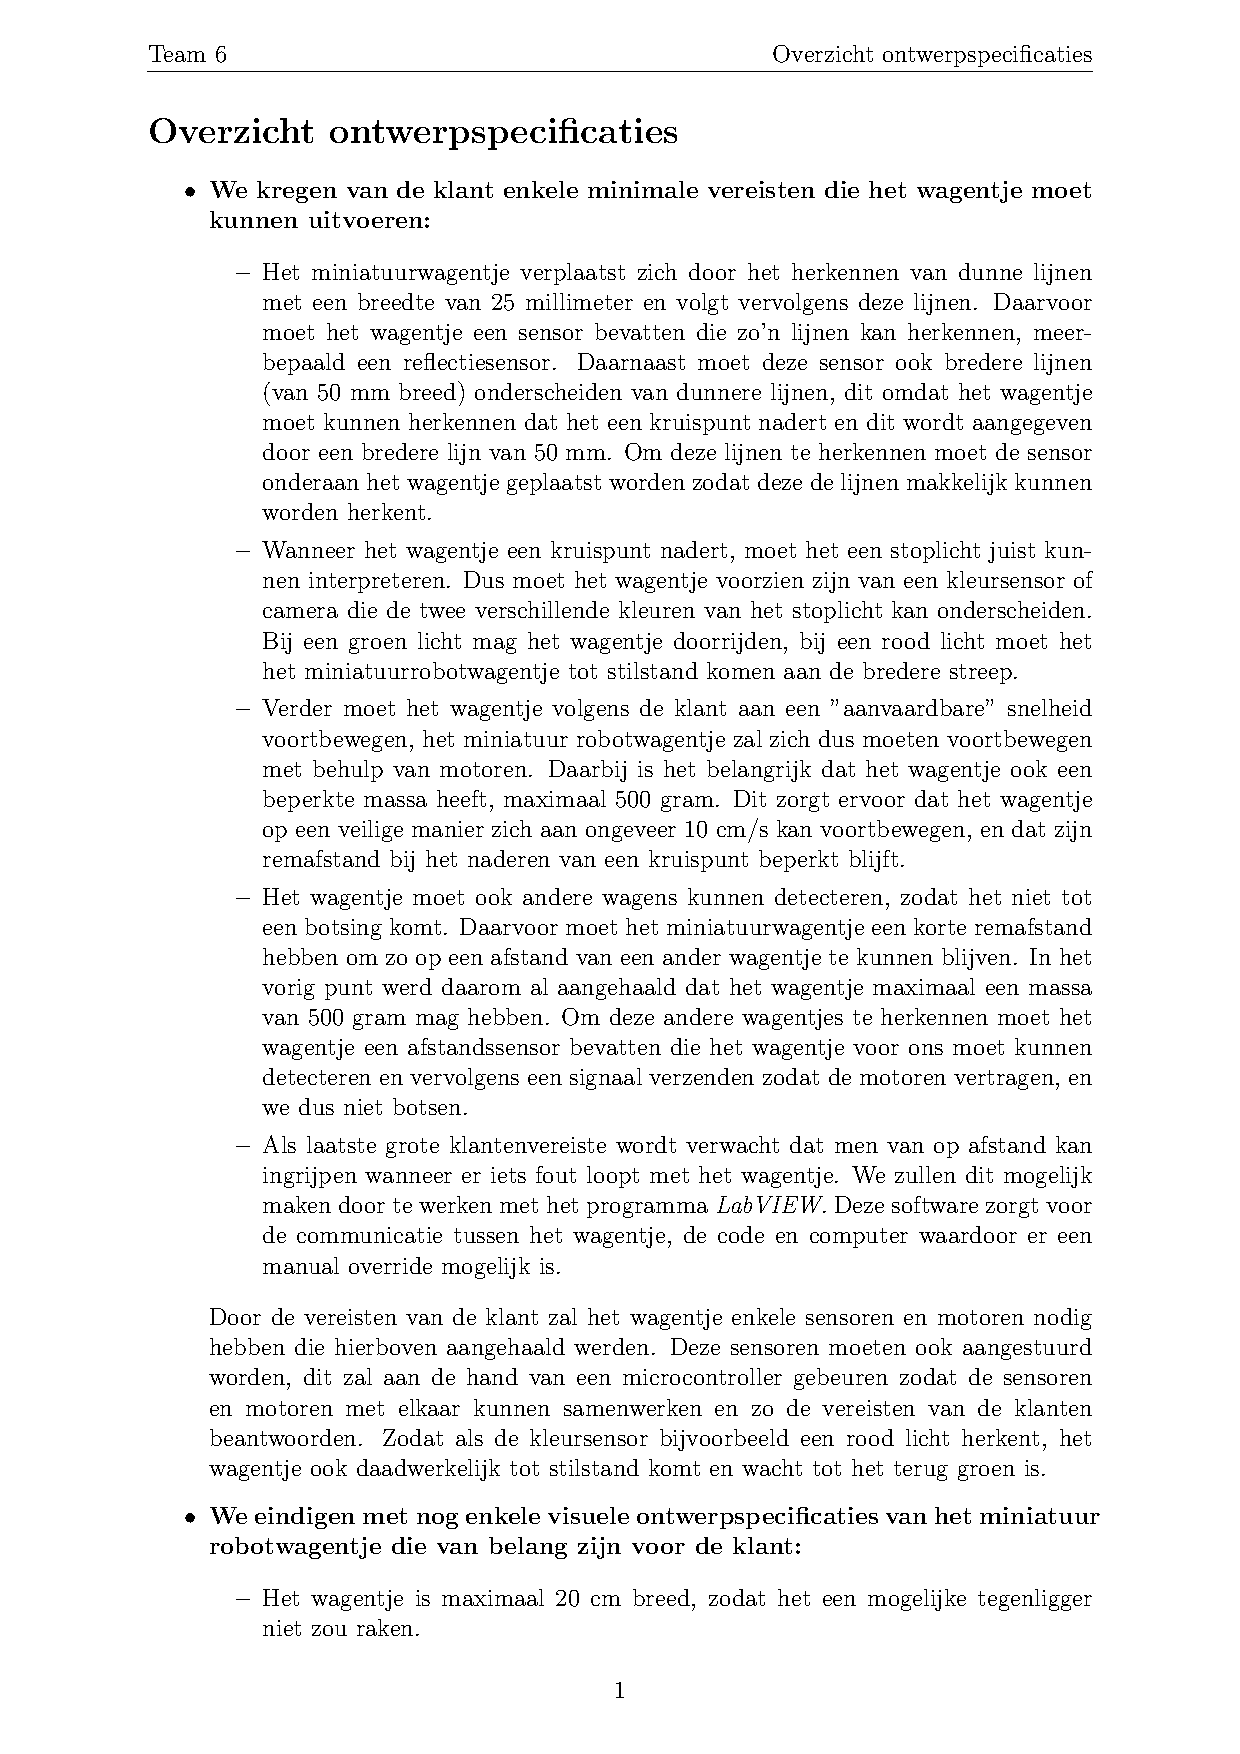
\includepdf[pages=-]{ontwerpspecificaties/ontwerpspecificaties.pdf}
	
	%\section*{Takenstructuur} % nog niet mooi weergegeven
	
\includepdf[pages=-]{taakstructuur/taakstructuur.pdf}
	
	%\section*{Verantwoordelijkheidsstructuur}
	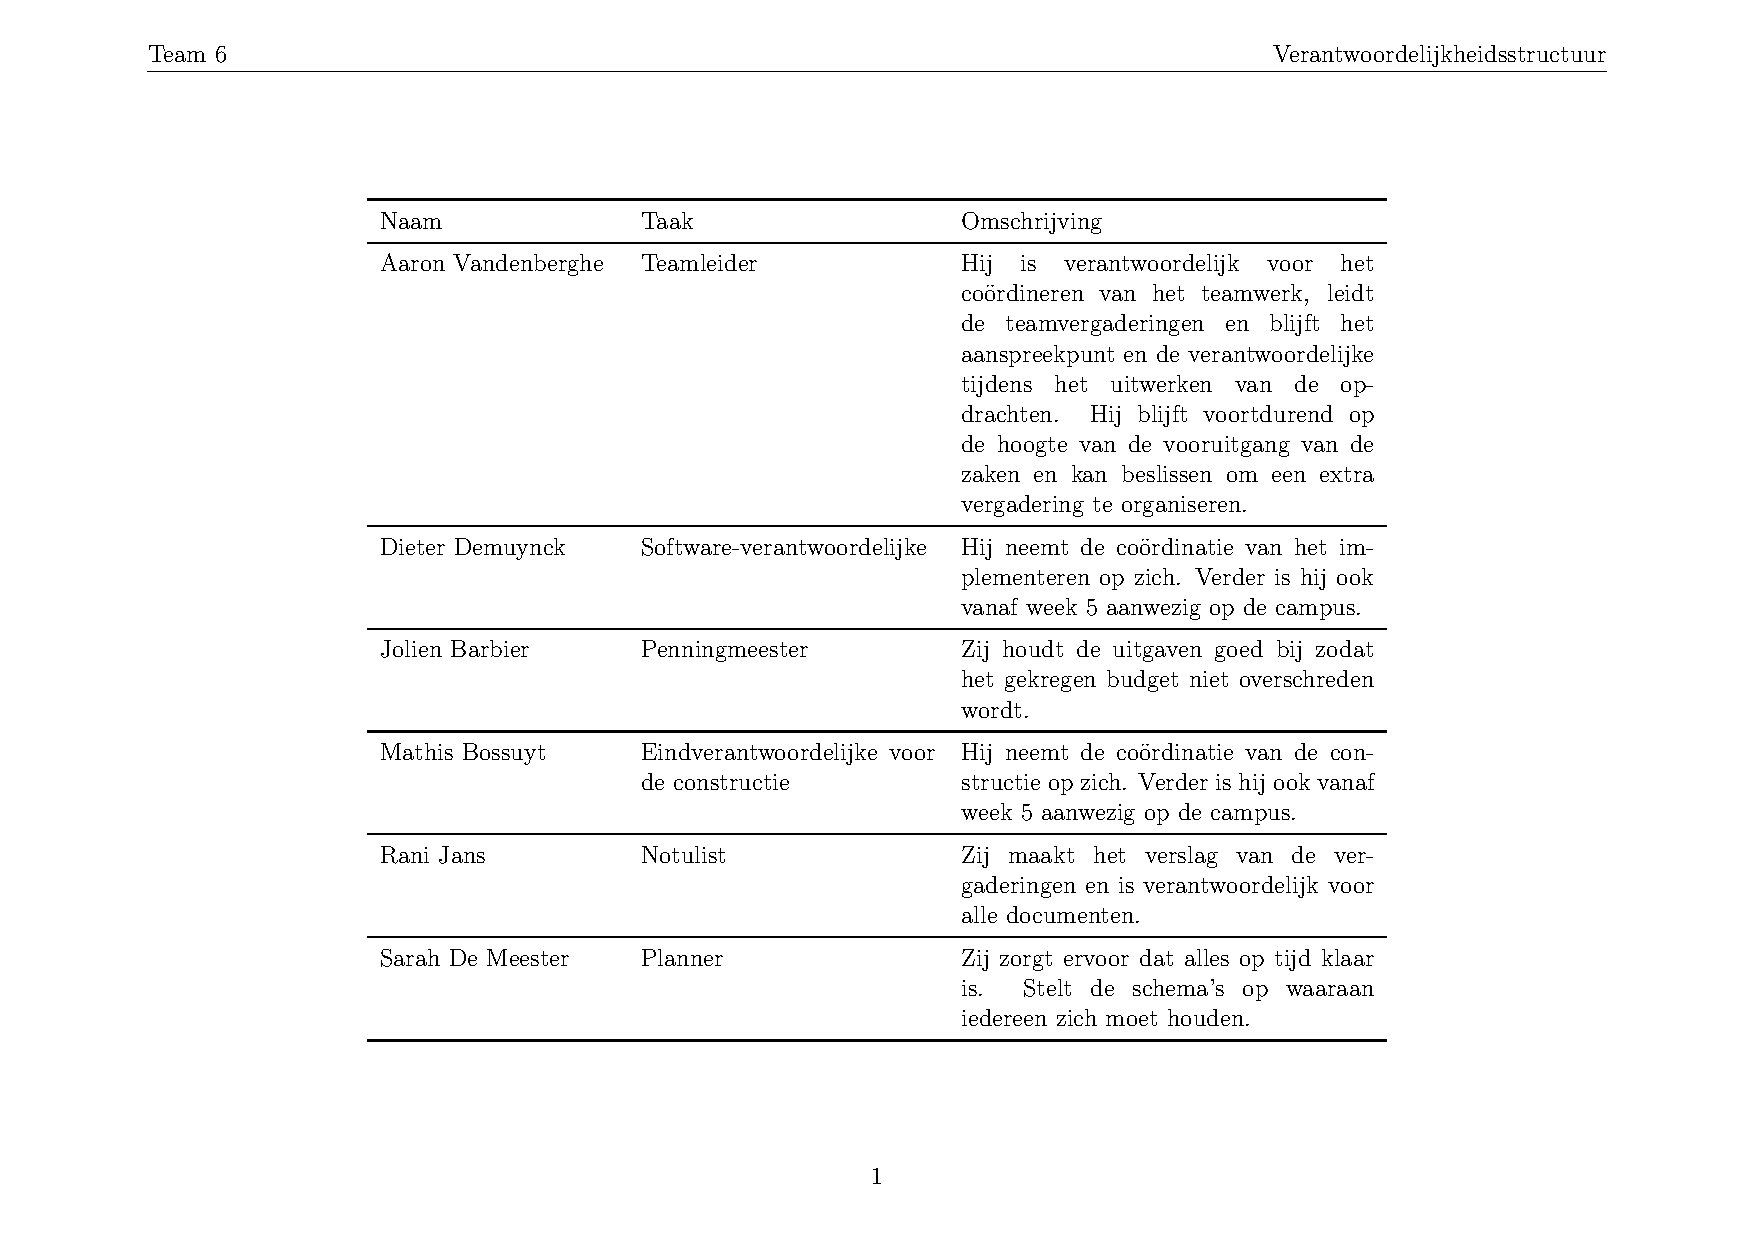
\includepdf[pages=-]{verantwoordelijkheidsstructuur/verantwoordelijkheidsstructuur.pdf}
	
	% teamkalender
	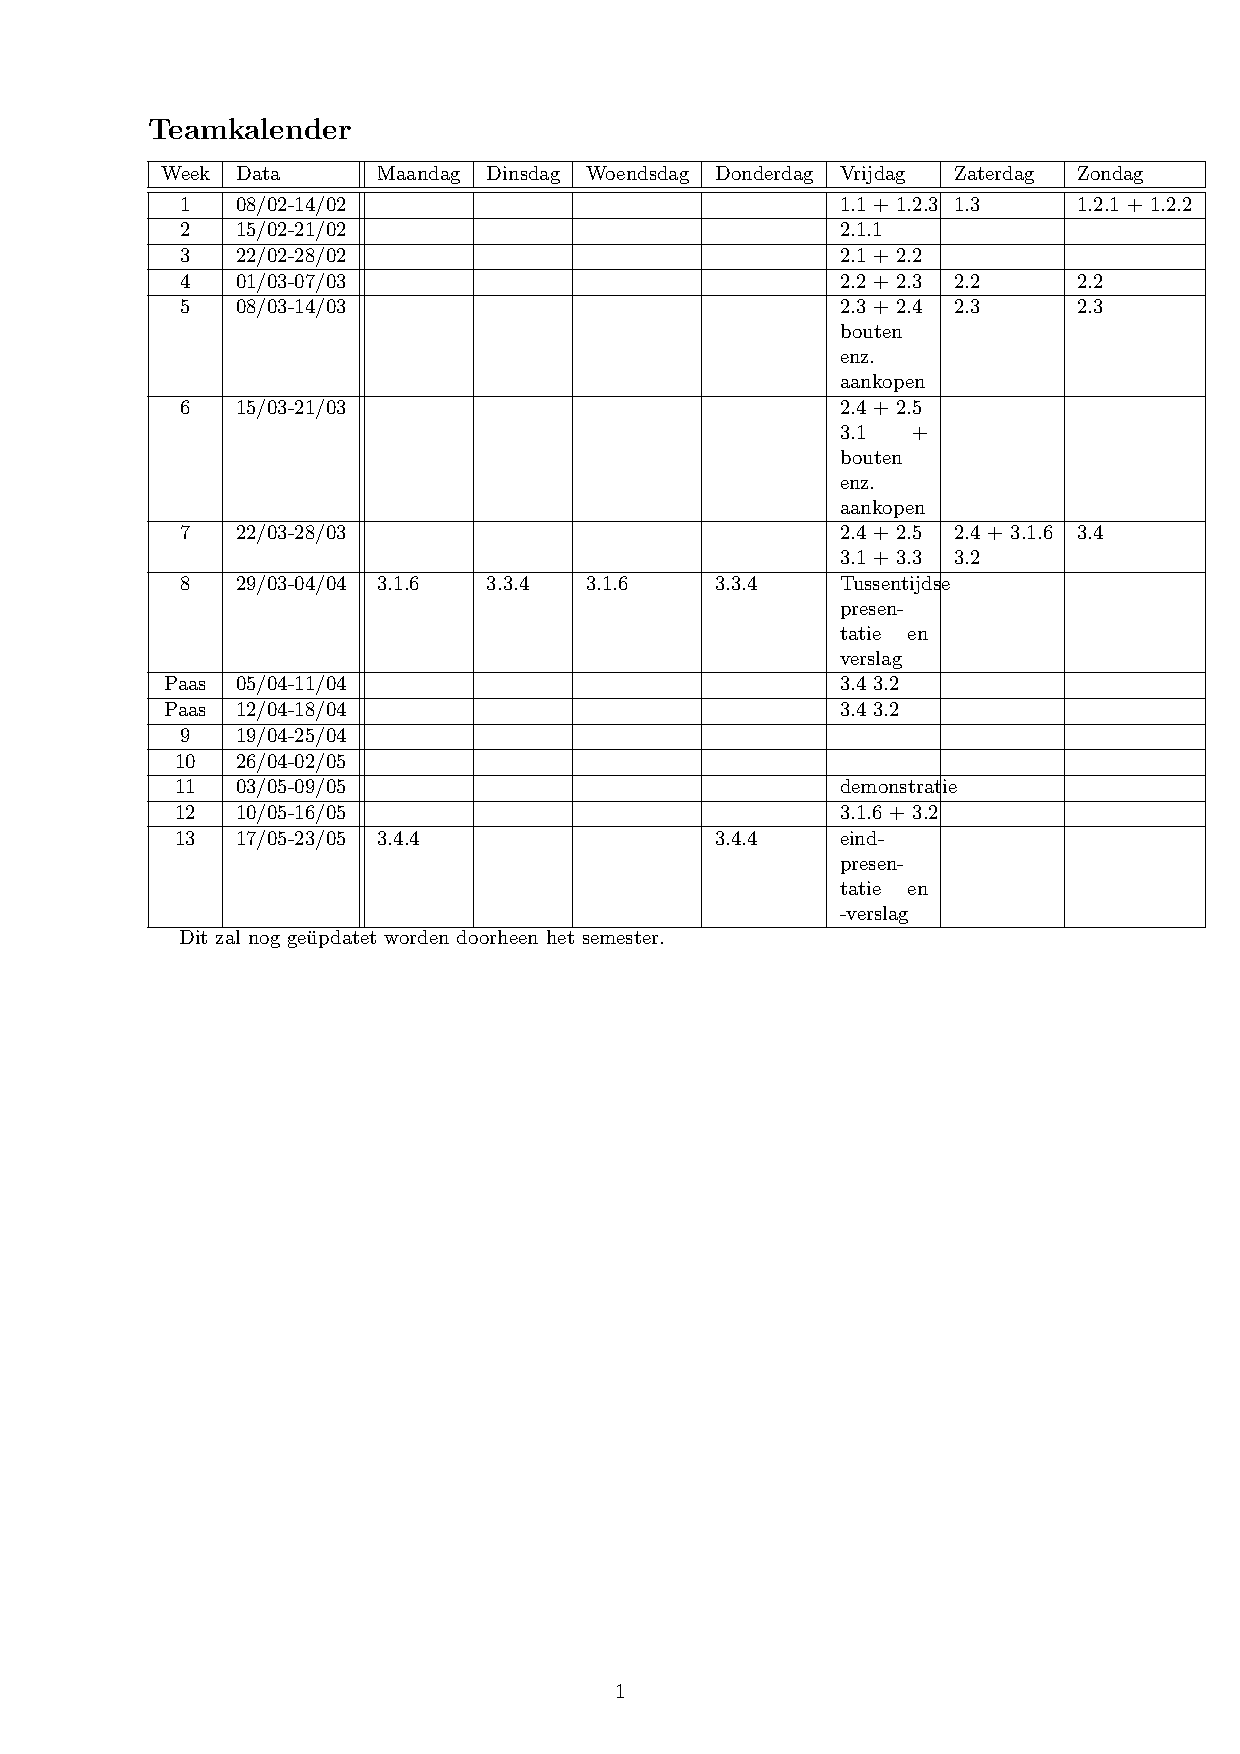
\includepdf[pages=-]{team6kalender/team6kalender.pdf}
	
	%\section*{Gannt-chart}	%nog niet mooi weergegeven
	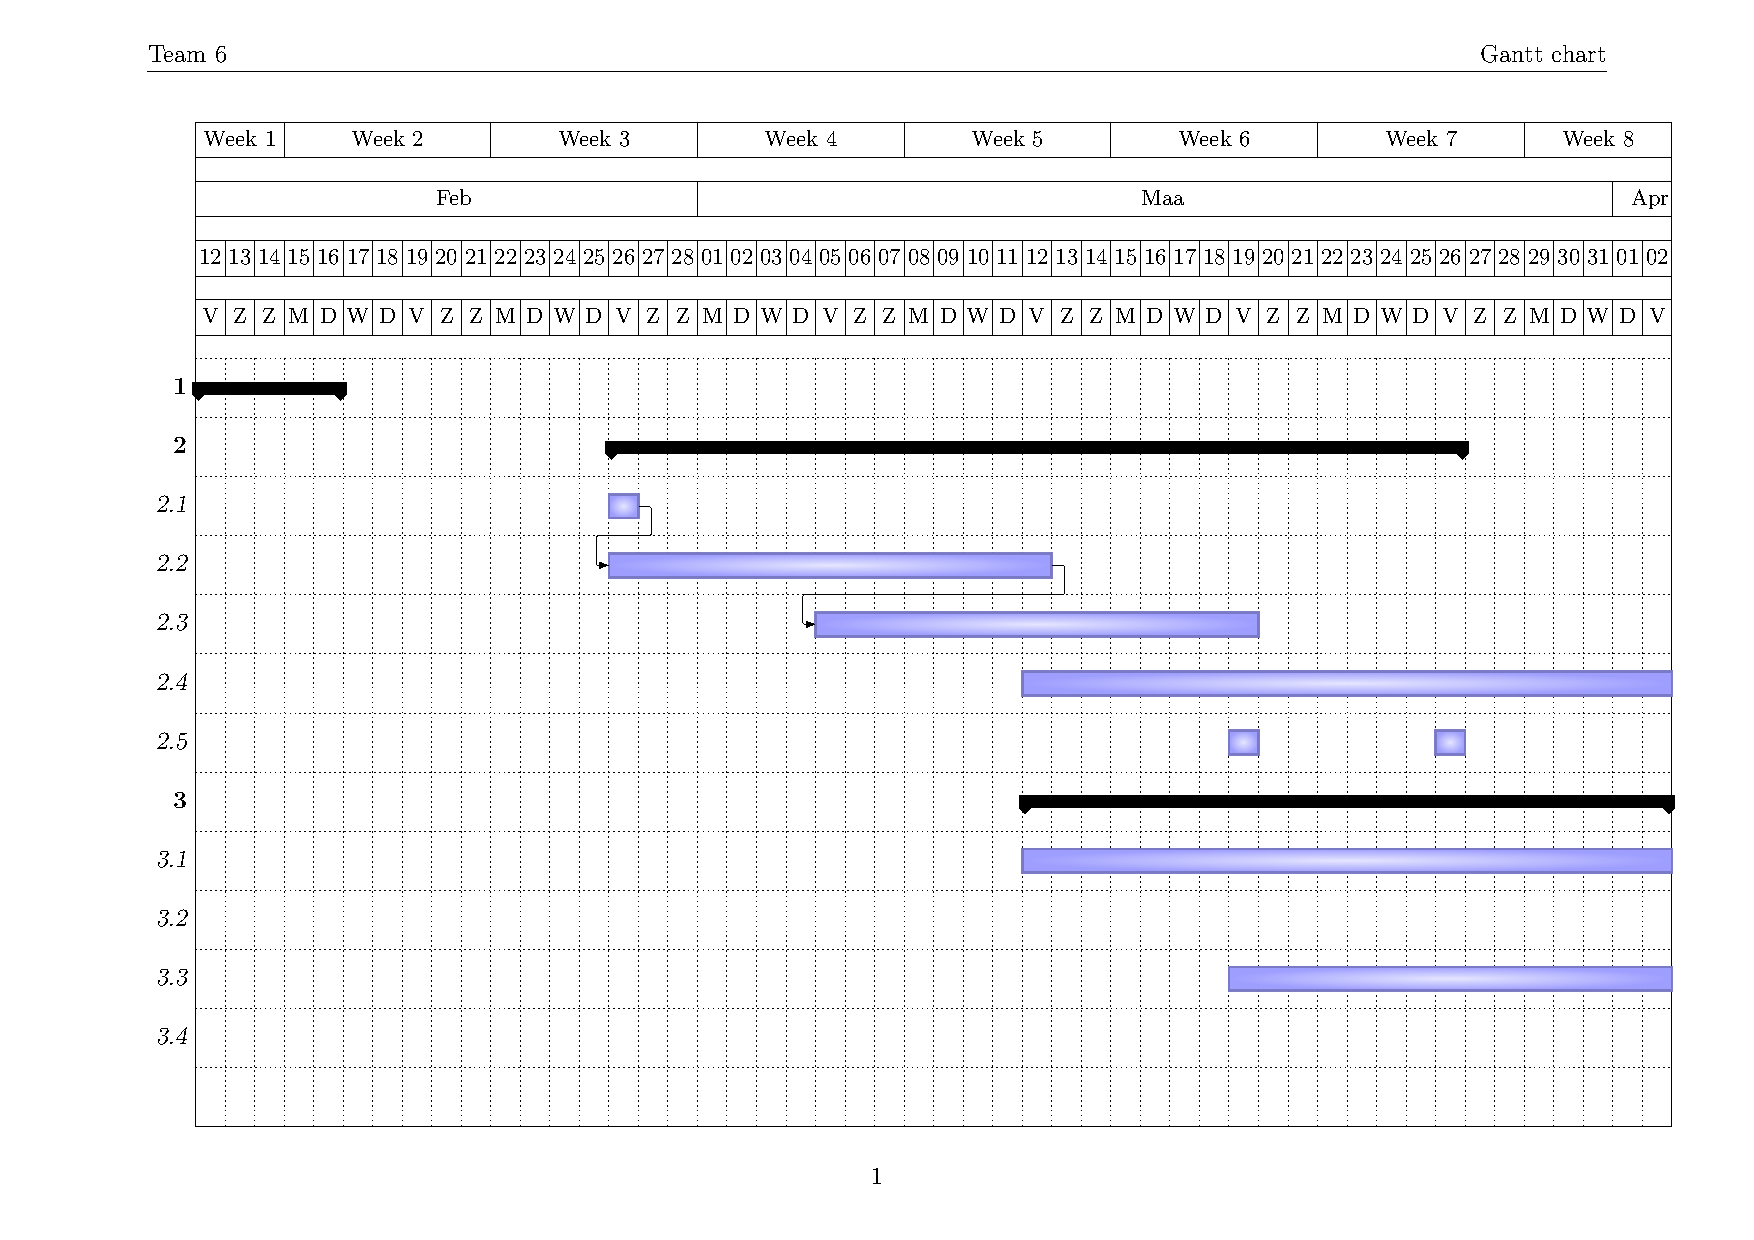
\includepdf[pages=-]{ganttchart/ganttchart.pdf}
\end{document}
